% 第1章第5节：空间之间的关系（包含关系与范数比较；换测度后的元素与范数；稠密子集与可分性；收敛方式与误差传递）。

\section{空间之间的关系}
\label{sec:fs-relations}

前两节分别构造了连续函数空间、$L^p$空间和数列空间。同一个函数常常同时属于几个空间，同一个误差也可以在几种范数下计算。本节分四个问题比较它们：成员能否从一个空间转入另一个空间；换一个测度后元素与范数怎样变化；能否用简单的、可数的对象逼近一般成员；以及不同意义下的收敛能互相推出什么。每个问题都先固定比较的对象，再给出足够的条件。

\subsection{包含关系与范数比较}
\label{sec:fs-inclusions}

\paragraph{有限测度下的包含}
在总测度有限的空间上，小范围的大值是影响可积性的主要因素，指数越高越难可积。

\begin{theorem}[有限测度下的$L^p$包含]
\label{thm:fs-lp-inclusion}
设$\mu(X)<\infty$，$1\leq p<q\leq\infty$。则$L^q(\mu)\subseteq L^p(\mu)$，并且对所有$f\in L^q(\mu)$，
\begin{equation}
 \|f\|_p\leq\mu(X)^{1/p-1/q}\,\|f\|_q ,
 \label{eq:fs-lp-inclusion}
\end{equation}
其中$q=\infty$时$1/q=0$。
\end{theorem}

\begin{proof}
设$q<\infty$。对$|f|^p\cdot1$使用Hölder不等式，指数取$r=q/p>1$与其共轭指数$r'=q/(q-p)$：
\[
 \int_X|f|^p\,d\mu\leq\Bigl(\int_X|f|^q\,d\mu\Bigr)^{p/q}\Bigl(\int_X1\,d\mu\Bigr)^{(q-p)/q}=\|f\|_q^p\,\mu(X)^{1-p/q}.
\]
两边开$p$次方即得式~\eqref{eq:fs-lp-inclusion}。$q=\infty$时直接由$|f|^p\leq\|f\|_\infty^p$几乎处处成立并积分，得$\|f\|_p\leq\mu(X)^{1/p}\|f\|_\infty$。
\end{proof}

\paragraph{计数测度下的反向包含}
在计数测度下，情况正好相反：总测度无限，但每个点的质量至少为$1$，不会出现“小范围的大值”，影响可求和性的是尾部衰减的快慢。对$p<q$，$\ell^p\subseteq\ell^q$且$\|x\|_q\leq\|x\|_p$。证明只需归一化：设$\|x\|_p=1$，则每个$|x_k|\leq1$，从而$|x_k|^q\leq|x_k|^p$，求和得$\|x\|_q^q\leq1$；一般情形由齐次性得到。

图~\ref{fig:fs-inclusions}把两种方向放在一起。在$(0,1]$上，$x^{-1/2}$可积但平方不可积（$\int_0^1x^{-1}\,dx$发散），$x^{-1/4}$平方可积但无界；在$\mathbb N_+$上，$(1/k)$平方可和但不可和，常数列有界但不平方可和。包含的方向取决于测度：有限测度下指数大的空间小，计数测度下指数小的空间小。在$\mathbb R$上的Lebesgue测度下，两个方向都不成立：$x^{-1/2}\mathbf 1_{(0,1]}$属于$L^1$而不属于$L^2$，$1/(1+|x|)$属于$L^2$（积分为$2$）而不属于$L^1$。

\begin{figure}[!htb]
  \centering
  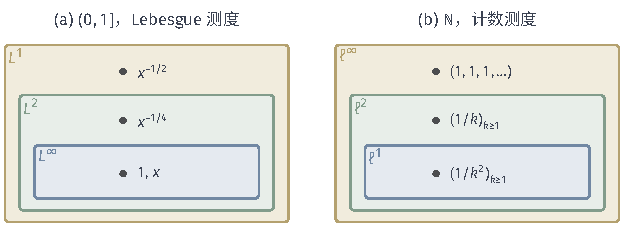
\includegraphics[width=105.7mm]{figures/02-abstract-mathematics/03-function-spaces/tikz/c1-inclusions/figure.pdf}
  \caption{两种测度下的包含方向，嵌套的框表示集合包含，点为各层之间的例子。(a)$(0,1]$上取Lebesgue测度，总质量有限：$L^\infty\subseteq L^2\subseteq L^1$，$x^{-1/4}$在$L^2$中但无界，$x^{-1/2}$可积但不平方可积。(b)$\mathbb N_+$上取计数测度：$\ell^1\subseteq\ell^2\subseteq\ell^\infty$，方向相反。}
  \label{fig:fs-inclusions}
\end{figure}

\paragraph{连续函数进入积分空间}
把一个连续函数“看作”$L^p$中的元素，实际上是一个映射。设$K$是紧度量空间，$\mu$是$K$上的有限Borel测度。连续函数有界且Borel可测，所以$\iota(f)=[f]_\mu$定义了线性映射$\iota:C(K)\to L^p(\mu)$，并且由定理~\ref{thm:fs-lp-inclusion}，
\[
 \|\iota(f)\|_p\leq\mu(K)^{1/p}\|f\|_\infty .
\]
这个映射不一定单射。若$\mu$是全支撑的，即每个非空开集的测度为正，则$f\neq g$时$\{f\neq g\}$是非空开集，测度为正，所以$\iota(f)\neq\iota(g)$。若$\mu$不是全支撑的，例如在$K=[0,1]$上令$\mu(A)$为$A\cap[0,\tfrac12]$的长度，则$f(x)=\max(0,x-\tfrac12)$是非零连续函数，而$\iota(f)=0$。所以只有核实了单射条件，才能把$C(K)$当作$L^p(\mu)$的子空间。

有限测度的假设也不能省。在$\mathbb R$上取Lebesgue测度，常数函数$1$属于$C_b(\mathbb R)$，却不属于任何$L^p$（$p<\infty$）。再取$h_n=\tfrac1n\mathbf 1_{[0,n^2]}$，有$\|h_n\|_\infty=\tfrac1n\to0$，而$\|h_n\|_2^2=\tfrac1{n^2}\cdot n^2=1$：高度在降低，支撑却在扩大，最大偏差趋于零不能推出平方积分误差趋于零。

\subsection{换测度后的元素与范数}
\label{sec:fs-change-of-measure}

同一个可测集合上换一个测度，首先改变的是“哪些差别不计”，其次才是误差的大小。设$\mu,\nu$是同一可测空间上的两个测度。若每个$\mu$零测集也是$\nu$零测集，称$\nu$关于$\mu$\term{绝对连续}（absolutely continuous），记作$\nu\ll\mu$；若两个方向都成立，称它们为\term{等价测度}（equivalent measures）。这些概念见第~\ref{sec:measure-absolute-continuity}节，Radon--Nikodym定理见第~\ref{sec:density-radon-nikodym}节。

\paragraph{零集关系与等价类}
若$\nu\ll\mu$，则$\mu$下几乎处处相等的两个函数在$\nu$下也几乎处处相等，所以$[f]_\mu\mapsto[f]_\nu$不依赖代表，是可测函数等价类之间良定义的线性映射。但它不一定是单射，也不一定保持可积性。

以$[0,1]$上的Lebesgue测度$\mu$与$d\nu=w\,d\mu$为例，其中$w\geq0$可测。由第~\ref{sec:density-weighted-measure}节，$\nu(A)=\int_Aw\,d\mu$是测度且$\nu\ll\mu$，并且$\int h\,d\nu=\int hw\,d\mu$对非负可测$h$成立。若$w=2\cdot\mathbf 1_{[0,1/2]}$，则$f=\mathbf 1_{(1/2,1]}$在$\mu$下不是零元素，在$\nu$下却是：新测度把原来不同的元素合并了。若$w>0$几乎处处，则$\mu\ll\nu$也成立，两个测度识别相同的零差别。

\paragraph{密度界与范数换算}
零集相同还不能保证误差可以互相控制，这需要密度的上下界。对$1\leq p<\infty$与可测函数$h$，
\[
 \|h\|_{L^p(\nu)}^p=\int_X|h|^p\,w\,d\mu .
\]
若$w\leq C$几乎处处，则$\|h\|_{L^p(\nu)}\leq C^{1/p}\|h\|_{L^p(\mu)}$，所以$L^p(\mu)$的成员都在$L^p(\nu)$中，$\mu$下的收敛推出$\nu$下的收敛。若还有$w\geq c>0$几乎处处，则$c^{1/p}\|h\|_{L^p(\mu)}\leq\|h\|_{L^p(\nu)}$，两个空间的成员相同，范数等价。

没有正下界时，反方向可能失败。取$w(x)=2x$与$f(x)=x^{-1/2}$，则
\[
 \int_0^1|f|^2\,d\mu=\int_0^1\frac{dx}{x}=\infty,\qquad \int_0^1|f|^2\,d\nu=\int_0^1\frac{1}{x}\cdot2x\,dx=2 .
\]
图~\ref{fig:fs-change-of-measure}显示了原因：$|f|^2=1/x$在$0$附近的面积无界，而权重$w=2x$恰好在那里趋于零，乘积是常数$2$。所以$f\in L^2(\nu)$但$f\notin L^2(\mu)$，尽管两个测度的零集相同。这里的$w\leq2$只给出$\|h\|_{L^2(\nu)}\leq\sqrt2\|h\|_{L^2(\mu)}$这一个方向。

\begin{figure}[!htb]
  \centering
  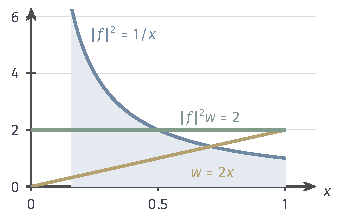
\includegraphics[width=58.1mm]{figures/02-abstract-mathematics/03-function-spaces/tikz/c1-change-of-measure/figure.pdf}
  \caption{换测度后的平方积分。$(0,1]$上$f(x)=x^{-1/2}$，$|f|^2=1/x$（蓝），其下方面积在$0$附近无界（阴影只画到$x=0.16$）；密度$w=2x$（黄）在$0$处趋于零，乘积$|f|^2w=2$（绿）的积分为$2$。所以$f\in L^2(w\,dx)$而$f\notin L^2(dx)$。}
  \label{fig:fs-change-of-measure}
\end{figure}

\paragraph{本质上界的换测度}
$L^\infty$只依赖零集，不需要密度界。若$\nu\ll\mu$，则$\{|f|>M\}$为$\mu$零测时也为$\nu$零测，所以$\|f\|_{L^\infty(\nu)}\leq\|f\|_{L^\infty(\mu)}$；若两个测度等价，本质上确界相同。把有限$p$的估计$C^{1/p}$令$p\to\infty$也能猜出这个结论，但它的成立靠的是零集关系，不是积分公式的极限。

\subsection{稠密子集与可分性}
\label{sec:fs-density-separability}

一般的$L^p$成员可能很不规则，计算和证明时常希望先对简单的函数验证，再推广到全空间。这要求简单函数能以任意精度逼近一般成员。度量空间中，若$D$的闭包是整个空间，称$D$\term{稠密}（dense）（定义~\ref{def:metric-separable}）。

\paragraph{简单函数的稠密性}
取值只有有限多个的可测函数称为简单函数。下面的定理说明，有限$p$的$L^p$中，支撑测度有限的简单函数已经足够。

\begin{theorem}[简单函数在$L^p$中稠密]
\label{thm:fs-simple-dense}
设$1\leq p<\infty$。形如$s=\sum_{i=1}^ka_i\mathbf 1_{A_i}$、其中$\mu(A_i)<\infty$的简单函数在$L^p(\mu)$中稠密。
\end{theorem}

\begin{proof}
先设$f\geq0$。取标准的二进逼近$s_n=\min\bigl(n,\,2^{-n}\lfloor2^nf\rfloor\bigr)$，它是简单函数，满足$0\leq s_n\leq f$且$s_n\uparrow f$逐点成立。于是$|f-s_n|^p\leq f^p$，后者可积，由控制收敛定理$\|f-s_n\|_p\to0$。每个$s_n$的非零取值至少为$2^{-n}$，而$\mu(\{s_n\geq2^{-n}\})\leq\mu(\{f\geq2^{-n}\})\leq2^{np}\|f\|_p^p<\infty$（最后一步是Chebyshev不等式），所以$s_n$的支撑测度有限。一般的$f$写成$f=f^+-f^-$，分别逼近后相减，由三角不等式即得。
\end{proof}

图~\ref{fig:fs-step-density}画出了$f(x)=\sin(\pi x)$的二进逼近。层高每减半一次，阶梯就更贴近曲线：$0\leq f-s_n<2^{-n}$，$n=2$时$L^2$误差约为$0.164$，$n=3$时约为$0.079$。这里$f$有界，所以截断$\min(n,\cdot)$不起作用；对无界的$f$，截断保证每个$s_n$只取有限多个值。

\begin{figure}[!htb]
  \centering
  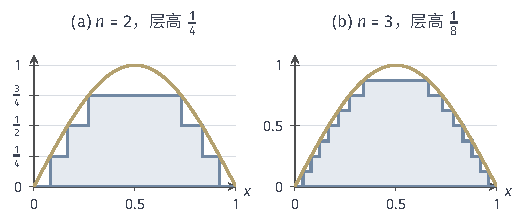
\includegraphics[width=88.7mm]{figures/02-abstract-mathematics/03-function-spaces/tikz/c1-step-density/figure.pdf}
  \caption{用二进简单函数逼近$f(x)=\sin(\pi x)$。$s_n=2^{-n}\lfloor2^nf\rfloor$在$f$落入$[k2^{-n},(k+1)2^{-n})$的位置取值$k2^{-n}$；(a)$n=2$，(b)$n=3$。逐点误差小于$2^{-n}$，$L^2([0,1])$误差约为$0.164$与$0.079$。}
  \label{fig:fs-step-density}
\end{figure}

\paragraph{连续紧支撑函数的稠密性}
在欧氏空间上，还可以用连续函数逼近。记$C_c(\Omega)$为开集$\Omega\subseteq\mathbb R^d$上支撑为紧集的连续函数。

\begin{theorem}[连续紧支撑函数在$L^p(\Omega)$中稠密]
\label{thm:fs-cc-dense}
设$\Omega\subseteq\mathbb R^d$为开集，取Lebesgue测度，$1\leq p<\infty$。则$C_c(\Omega)$在$L^p(\Omega)$中稠密。
\end{theorem}

\begin{proof}
由定理~\ref{thm:fs-simple-dense}和三角不等式，只需逼近有限测度可测集$A\subseteq\Omega$的示性函数。由Lebesgue测度的正则性，对$\varepsilon>0$存在紧集$K$与开集$U$，使$K\subseteq A\subseteq U\subseteq\Omega$且$\lambda(U\setminus K)<\varepsilon$；缩小$U$还可使其闭包是$\Omega$中的紧集。令
\[
 \varphi(x)=\frac{\operatorname{dist}(x,U^c)}{\operatorname{dist}(x,U^c)+\operatorname{dist}(x,K)} .
\]
分母处处为正，$\varphi$连续，在$K$上等于$1$、在$U$外等于$0$、取值在$[0,1]$中，所以$\varphi\in C_c(\Omega)$。$\mathbf 1_A-\varphi$只在$U\setminus K$上非零且绝对值不超过$1$，故$\|\mathbf 1_A-\varphi\|_p^p\leq\lambda(U\setminus K)<\varepsilon$。
\end{proof}

取$\Omega=\mathbb R^d$，定理~\ref{thm:fs-cc-dense}特别给出：$C_c(\mathbb R^d)$在$L^p(\mathbb R^d)$（$1\leq p<\infty$）中稠密。

同样的“先逼近示性函数、再用距离函数构造连续过渡”的论证不依赖欧氏结构，只需测度能被闭集和开集从内外逼近。度量空间上的有限Borel测度具有这种正则性：对每个Borel集$A$与$\varepsilon>0$，存在闭集$F$与开集$U$，使$F\subseteq A\subseteq U$且$\mu(U\setminus F)<\varepsilon$。由此得到紧度量空间上的版本。

\begin{theorem}[紧度量空间上连续函数的稠密性]
\label{thm:fs-continuous-dense-compact}
设$K$为紧度量空间，$\mu$为$K$上的有限Borel测度，$1\leq p<\infty$。则$\{[f]_\mu:f\in C(K)\}$在$L^p(\mu)$中稠密。
\end{theorem}

\begin{proof}
由定理~\ref{thm:fs-simple-dense}，只需逼近Borel集$A$的示性函数。按上面的正则性取闭集$F\subseteq A\subseteq U$（$U$开，$\mu(U\setminus F)<\varepsilon$），定义与定理~\ref{thm:fs-cc-dense}证明中相同的$\varphi$，只把$K$换成$F$。$F$闭、$U^c$闭且二者不交，所以分母处处为正，$\varphi$连续，在$F$上为$1$、在$U$外为$0$，于是$\|\mathbf 1_A-\varphi\|_p^p\leq\mu(U\setminus F)<\varepsilon$。$U=K$或$F=\varnothing$时分别取$\varphi\equiv1$或$\varphi\equiv0$即可。
\end{proof}

\paragraph{区间阶梯函数的稠密性}
在$L^2(0,1)$中，比连续函数更简单的区间阶梯函数也已足够。所谓区间阶梯函数，是有限个区间示性函数的线性组合。给定$f\in L^2(0,1)$与$\varepsilon>0$，由定理~\ref{thm:fs-cc-dense}取连续函数$g$使$\|f-g\|_2<\varepsilon$；$g$在$[0,1]$上一致连续（定理~\ref{thm:metric-compact-uniform}），取$m$足够大，使每个长为$1/m$的区间上$g$的振幅小于$\varepsilon$，令$s$在$[(j-1)/m,j/m)$上取常数$g(j/m)$，则$\|g-s\|_\infty\leq\varepsilon$，从而$\|g-s\|_2\leq\varepsilon$。合起来$\|f-s\|_2<2\varepsilon$。所以区间阶梯函数在$L^2(0,1)$中稠密；同样的论证对任意有限$p$成立。

这些结论回答了斜坡例子留下的问题。$C([-1,1])$在$L^2([-1,1])$中稠密，而$L^2([-1,1])$完备，所以$L^2([-1,1])$正是$(C([-1,1]),\|\cdot\|_2)$的完备化：第~\ref{sec:fs-banach}小节抽象构造出来的“新元素”，在这里被识别为平方可积函数的等价类。用光滑函数逼近需要卷积平滑，留到第~\ref{sec:sob-mollification}小节。

\paragraph{可分性}
稠密子集可以很大。若一个空间有可数的稠密子集，称它\term{可分}（separable）（定义~\ref{def:metric-separable}）。可分空间中的每个元素都能用可数多个“标准对象”中的某些去逼近，这在构造可数正交基、对角线抽取子列时都要用到。

$C([a,b])$可分。Weierstrass逼近定理断言多项式在$(C([a,b]),\|\cdot\|_\infty)$中稠密，证明见第~\ref{sec:apx-polynomial}小节；把多项式的系数换成有理数，误差可以任意小，而有理系数多项式只有可数多个。$\ell^p$（$1\leq p<\infty$）可分：只有有限个非零项且各项为有理数的数列可数，截断尾部和把各项换成有理数都只产生任意小的误差。$L^p(\Omega)$（$1\leq p<\infty$）也可分：由定理~\ref{thm:fs-cc-dense}，可以先用连续紧支撑函数逼近，再在其支撑上用有理系数多项式一致逼近，并乘以有理顶点方体的示性函数（其细节与上面的证明类似，这里从略）。

可数稠密子集与有限维基是两回事。$C([a,b])$中的有理系数多项式可数且稠密，但$e^x$不是其中任何一个的有限线性组合；可分只说明每个元素是可数集合中元素的极限，不说明它能用有限多个方向精确表示。

可分性也不是所有函数空间的共同性质。在$L^\infty([0,1])$中取$f_t=\mathbf 1_{[0,t]}$，$t\in[0,1]$。对$s<t$，$f_t-f_s=\mathbf 1_{(s,t]}$在正测度集上等于$1$，所以$\|f_t-f_s\|_\infty=1$。以每个$f_t$为中心、半径$\tfrac12$的开球两两不交，共有不可数个；若$D$稠密，每个球中至少有$D$的一个元素，且这些元素各不相同，所以$D$不可数。故$L^\infty([0,1])$不可分。同样的论证用于$0$--$1$数列，说明$\ell^\infty$不可分。

\subsection{收敛方式与误差传递}
\label{sec:fs-convergence-modes}

函数列可以在多种意义下收敛。本小节先说明怎样用范数不等式把一种收敛传给另一种，再用三个对照序列标出不能推出的边界。

\paragraph{用范数不等式传递收敛}
设同一线性空间上有两个范数，且存在与序号无关的常数$C$，使$\|h\|_A\leq C\|h\|_B$对所有$h$成立。对$h=f_n-f$使用这个不等式，$\|f_n-f\|_B\to0$即推出$\|f_n-f\|_A\to0$。若两个方向都有这样的常数，两种收敛等价。关键在于常数不随$n$变化，并且两个范数作用于同一列函数、同一个候选极限。

由定理~\ref{thm:fs-lp-inclusion}，在有限测度空间上，$L^q$收敛推出$L^p$收敛（$p<q$），一致收敛推出每个$L^p$收敛。$\mathbb R$上$h_n=\tfrac1n\mathbf 1_{[0,n^2]}$的例子说明，测度无限时后一结论失效。

\paragraph{三个对照序列}
图~\ref{fig:fs-convergence-modes}和表~\ref{tab:fs-convergence-modes}对照了$[0,1]$上Lebesgue测度下的三个序列。

\begin{figure}[!htb]
  \centering
  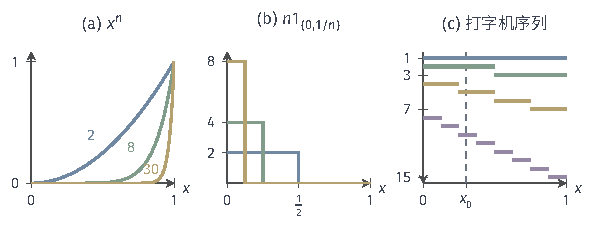
\includegraphics[width=100.4mm]{figures/02-abstract-mathematics/03-function-spaces/tikz/c1-convergence-modes/figure.pdf}
  \caption{三种收敛方式的反例。(a)$x^n$，$n=2,8,30$：逐点趋于端点处为$1$、其余为$0$的函数，$L^p$范数趋于零，最大偏差恒为$1$。(b)窄尖峰$n\mathbf 1_{(0,1/n)}$，$n=2,4,8$：每一点最终为零，积分却恒为$1$。(c)打字机序列的前$15$项，第$k$层把$[0,1)$等分为$2^k$段，依次取各段的示性函数；纵轴为项号，横条为支撑。竖虚线$x=x_0$在每一层恰好穿过一个横条。}
  \label{fig:fs-convergence-modes}
\end{figure}

\begin{table}[!htb]
  \centering
  \begin{tabular}{@{}lccc@{}}
    \toprule
    序列 & 逐点收敛到$0$ & $L^1$收敛到$0$ & 一致收敛到$0$ \\
    \midrule
    $x^n$ & 除$x=1$外 & 是 & 否 \\
    $n\mathbf 1_{(0,1/n)}$ & 是（处处） & 否 & 否 \\
    打字机序列 & 处处不收敛 & 是 & 否 \\
    \bottomrule
  \end{tabular}
  \caption{$[0,1]$上Lebesgue测度下三个序列的收敛性质。}
  \label{tab:fs-convergence-modes}
\end{table}

$x^n$的计算已在第~\ref{sec:fs-lp}小节完成：$\|x^n\|_p=(np+1)^{-1/p}\to0$，逐点极限在$x=1$处为$1$，但这只是一个零测点，所以作为$L^p$元素，逐点极限与零元素相同，两种说法并不矛盾。最大偏差恒为$1$，不一致收敛。

窄尖峰$g_n=n\mathbf 1_{(0,1/n)}$在每个$x$处最终为零：$x\leq0$时恒为零，$x>0$时只要$n>1/x$就有$g_n(x)=0$。但$\|g_n\|_1=1$，$\|g_n\|_2=\sqrt n\to\infty$。逐点收敛允许不同位置在不同时刻进入误差带，因而管不住越来越窄、越来越高的峰。

\begin{example}[打字机序列]
\label{ex:fs-typewriter}
对$k=0,1,2,\ldots$与$j=0,\ldots,2^k-1$，令$h_{k,j}=\mathbf 1_{[j2^{-k},(j+1)2^{-k})}$，并按$k$从小到大、同一层内按$j$从小到大排成一列：$h_{0,0},h_{1,0},h_{1,1},h_{2,0},\ldots$。第$k$层每一项的范数是$\|h_{k,j}\|_p=2^{-k/p}$，随项号增大趋于零，所以序列在每个$L^p$（$p<\infty$）中收敛到$0$。但对每个$x_0\in[0,1)$，每一层恰好有一项在$x_0$处取$1$，其余项取$0$，所以数列$(h_{k,j}(x_0))$中$0$和$1$都出现无穷多次，在任何一点都不收敛。
\end{example}

\paragraph{子列与控制条件}
打字机序列说明$L^p$收敛推不出整列的逐点收敛，但定理~\ref{thm:fs-ae-subsequence}保证可以抽出几乎处处收敛的子列。这里可以直接写出一个：子列$h_{k,0}=\mathbf 1_{[0,2^{-k})}$对每个$x>0$在$2^{-k}<x$后恒为零，所以它在$(0,1]$上逐点收敛到$0$，例外只有零测点$x=0$。

反方向，从几乎处处收敛推出$L^p$收敛需要附加条件。若$f_n\to f$几乎处处，且存在同一个$G\in L^p$使$|f_n|\leq G$几乎处处对所有$n$成立，则$|f|\leq G$，$|f_n-f|^p\leq2^pG^p$可积，由控制收敛定理$\|f_n-f\|_p\to0$。窄尖峰没有这样的控制函数：$\sup_ng_n(x)$在$x\in[\tfrac1{n+1},\tfrac1n)$上至少为$n$，大于$\tfrac1x-1$，不可积。所以“每项各自可积”不能代替“同一个可积函数控制所有项”。

\paragraph{弱收敛的预告}
还有一种收敛不要求整体误差趋于零。在$L^2(0,2\pi)$中取$u_n(x)=\sin(nx)$，有$\|u_n\|_2^2=\pi$，序列不趋于零。但对任意区间$[a,b]\subseteq[0,2\pi]$，
\[
 \int_0^{2\pi}\sin(nx)\,\mathbf 1_{[a,b]}(x)\,dx=\frac{\cos(na)-\cos(nb)}{n}\to0 :
\]
与每个固定的阶跃函数比较，$u_n$越来越接近零函数。这种“通过每个固定的连续线性读取来判断极限”的收敛称为弱收敛，它需要先建立线性泛函，正式定义见第~\ref{sec:lfo-weak-convergence}小节。它与概率测度的弱收敛（第~\ref{sec:wlim-weak-convergence}节）名字相同，但变化的对象与测试对象都不同，不能互换。
